\vspace{2cm}
\rhead{SENSITIVITY ANALYSIS}
\chapter{Introduction}
\lhead{Introduction}
Sensitivity analysis (SA) studies how changes in the input of a model affect the output, and it is essential for many engineering applications, such as uncertainty quantification, optimal design, and to answer \textit{what if} questions, i.e. what happens to the solution of the model if the input parameters change. These tasks can be performed in many different ways, depending on the nature of the model considered. In this work, we consider systems that can be modelled with partial differential equations (PDEs). The sensitivity variable itself is defined as the derivative of the state (i.e., the output of the model) with respect to the parameters of interest. 

In the framework of PDEs, one can distinguish two main classes of methods: the \textit{differentiate-then-discretise} methods and the \textit{discretise-then-differentiate} methods. As the names say, in the first case the state model is formally differentiated with respect to the parameter of interest, providing an analytical sensitivity system which can then be discretised with the most appropriate numerical scheme. The second class of methods swaps the two steps which, in the general case, are not commutative. A detailed comparison between the two classes of methods can be found in \cite{gunzburger2003perspectives} for optimisation problems. 
In this work, we focus on the first class, and, in particular, on the continuous sensitivity equation method \cite{Borggaard1997366,duvigneau2006improved,Duvigneau_Pelletier_06_ijcfd,chalons2018sensitivity, SA_Euler}.

The main aim of this work is to give an estimate of the variance of the solution of the Navier--Stokes equations when there are uncertain parameters and then to use the estimated variance to compute confidence intervals. This goes under the name of forward uncertainty propagation, which is part of the broader field of uncertainty quantification (UQ). Many strategies and techniques have been proposed in the literature to tackle UQ problems, particularly in the case of PDEs models: Monte Carlo method \cite{christian1999monte}, polynomial chaos \cite{Walters_03, Xiu_et_Karniadakis_03, Knio_LeMaitre_06, Despres2013}, random space partition \cite{abgrall_congedo_13}, to name but a few. A review of these methods applied to fluid dynamics problems can be found in \cite{walters2002uncertainty}. 

Methods of uncertainty propagation based on SA are particularly efficient in terms of computational time if compared, for instance, to methods like Monte Carlo. However, since SA is based on Taylor expansions of the state variable with respect to the parameter of interest, these methods are intrinsically local \cite{delenne2014propagation}~: they can be used only for random variables with a small variance. The Monte Carlo approach does not require this assumption; however, it is not applicable for realistic unsteady test cases in $2D$ and $3D$, due to its high computational cost. In this work we propose an approach based on the sensitivity equation method: under the hypothesis of small variance of the input parameters, we can provide a first-order estimate of the variance of the solution at a reasonable computational cost. 
\newpage
\rhead{SENSITIVITY ANALYSIS}
\chapter{The physical model}
\lhead{The physical model}
\label{sec_physical_model}
In this section, we present the physical model and its sensitivity. A more detailed description can be found in~\cite{FDP20}.
\section{The state equations}
Let us consider the domain $\Omega$ in Figure~\ref{domain}: it is a channel with walls on the top and the bottom and an obstacle of square section at distance $x_D$ from the inflow boundary. The Navier-Stokes system and the boundary conditions for this domain are:
\begin{figure}[h]
\begin{center}
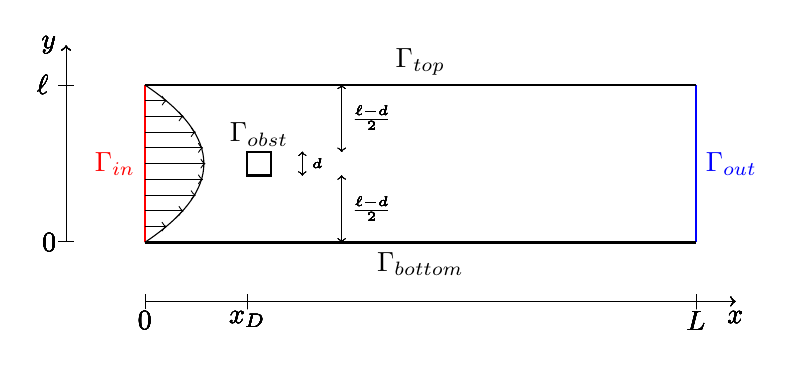
\begin{tikzpicture}
\draw[thick, red] (0,0) -- (0,2);
\draw[thick, blue] (7,0) -- (7,2);
\draw[thick] (1.3,0.85) rectangle (1.6,1.15);
\draw[thick] (0,0) -- (7,0);
\draw[thick] (0,2) -- (7,2);
\node[left] at (0,1) {\color{red}$\Gamma_{in}$};
\node[right] at (7,1) {\color{blue}$\Gamma_{out}$};
\node[above] at (3.5,2) {$\Gamma_{top}$};
\node[below] at (3.5,0) {$\Gamma_{bottom}$};
\node[above] at (1.45,1.1) {$\Gamma_{obst}$};
\draw[thin] (0,0) .. controls (1,2/3) and (1, 4/3) .. (0,2);
\foreach \y in {2, 4, ..., 18}{
\draw[thin,->] (0,0.1*\y) -- (0.2*\y*0.77-0.01*\y*\y*0.77,0.1*\y);
%asse y
\draw[thin,|->] (-1,0)--(-1,2.5);
\draw[very thin] (-1.1,2)--(-0.9,2);
\node[left] at (-1,0) {$0$};
\node[left] at (-1.1,2) {$\ell$};
\node[left] at (-1,2.5) {$y$};
%asse x
\draw[thin,|->] (0,-.75)--(7.5,-.75);
\draw[very thin] (1.3,-.85)--(1.3,-0.65);
\draw[very thin] (7,-.85)--(7,-0.65);
\node[below] at (0,-.75) {$0$};
\node[below] at (1.3,-.75) {$x_D$};
\node[below] at (7,-.75) {$L$};
\node[below] at (7.5,-.75) {$x$};
%misura e posizione ostacolo
\draw[very thin, <->] (2, 0.85)--(2, 1.15);
\node[right] at (2,1) {\tiny $d$};
\draw[very thin, <->] (2.5, 0)--(2.5, 0.85 );
\node[right] at (2.5,0.425) {\tiny $\frac{\ell-d}{2}$};
\draw[very thin, <->] (2.5, 1.15)--(2.5, 2);
\node[right] at (2.5,1.575) {\tiny $\frac{\ell-d}{2}$};
}
\end{tikzpicture}
\caption{Domain for the first test case.}
\label{domain}
\end{center}
\end{figure}

\begin{equation}
\begin{cases}
\partial_t \b_u - \nu \Delta \b_u + (\b_u \cdot \nabla) \b_u + \nabla p = \mathbf{f}& \Omega, t > 0, \\
\nabla \cdot \b_u = 0 & \Omega, t>0, \\
\b_u (\mathbf{x}, 0) = 0 & \Omega, t=0, \\
\b_u = - g(y)\mathbf{n} & \text{on } \Gamma_{in}, \\
\b_u = 0 & \text{on } \Gamma_w = \Gamma_{obst} \cup \Gamma_{top} \cup \Gamma_{bottom}, \\
(\nu \nabla \b_u -pI) \mathbf{n} = 0 & \text{on } \Gamma_{out},
\end{cases}
\label{state}
\end{equation}
where $\b_u = (u^x, u^y)^t$ is the velocity, $p$ is the pressure, $\mathbf{f}$ the external force and $g(y)$ the prescribed inflow condition. The first equation models the conservation of the momentum and the second one the conservation of the mass. In the following, they will be referred to as, respectively, the momentum equation and the mass equation. We impose no slip boundary condition of the walls of the domain, a prescribed velocity at the inflow and a homogeneous Neumann boundary condition at the outflow. 


\section{The sensitivity equations}
We now consider $\b_u$ as a function of space, time and a scalar uncertain parameter $a$, $\b_u = \b_u(\mathbf{x},t;a)$ and we write a formal Taylor expansion with respect to $a$:
\begin{equation}
\b_u(\mathbf{x},t;a+\delta a) = \displaystyle \sum_{k=0}^\infty \b_u_k(\mathbf{x},t;a) \delta a^k,
\label{series}
\end{equation}
where $\b_u_0 = \b_u$ and the coefficient $\b_u_k$ is the $k-$th derivative of $\b_u$ with respect to $a$:
\[
\b_u_k(\mathbf{x},t;a) := \frac{d^k}{da^k} \b_u(\mathbf{x},t;a),
\]
and it is called the $k-$th order sensitivity. To consider more than one parameter of interest, the sensitivity should be defined as the gradient of the state with respect to the vector of parameters and a multi-dimensional Taylor expansion would be necessary, but this is not treated in this work. A similar expansion can be done for the pressure $p$, and the data $\mathbf{f}$, $\mathbf{d}$, and $g$. In order to write the equations for the sensitivities, one can replace (\ref{series}) into (\ref{state}) and then factorise according to the powers of $\delta a$. For $k=0$ we obtain the state system (\ref{state}). For $k=1$, we obtain the first order sensitivity equations. In this work, we consider only first-order sensitivity and the notation $\b_u_1 = \b_u_a$ will be employed. This choice is common \cite{Borggaard1997366, duvigneau2006improved, Duvigneau_Pelletier_06_ijcfd, chalons2018sensitivity, SA_Euler} because in most cases first order sensitivities provide enough information. It is possible to consider higher order sensitivities if necessary, but this is not investigated in this work. The first order sensitivity equations, referred to as the sensitivity equations in short, are:
\begin{equation}
\begin{cases}
\partial_t \b_u_a - \nu \Delta \b_u_a + (\b_u_a \cdot \nabla) \b_u + (\b_u \cdot \nabla) \b_u_a + \nabla p_a = \mathbf{f}_a& \Omega, t > 0, \\
\nabla \cdot \b_u_a = 0 & \Omega, t>0, \\
\b_u_a (\mathbf{x}, 0) = 0 & \Omega, t=0, \\
\b_u_a = - g_a(y)\mathbf{n} & \text{on } \Gamma_{in}, \\
\b_u_a = 0 & \text{on } \Gamma_w , \\
(\nu \nabla \b_u_a -p_aI) \mathbf{n} = 0 & \text{on } \Gamma_{out},
\end{cases}
\label{sensitivity}
\end{equation}
where $\Gamma_w := \Gamma_{obst} \cup \Gamma_{top} \cup \Gamma_{bottom}$.
These are known as the Oseen equations: an introduction on the subject can be found in \cite{john2014oseen}, both for the theoretical and the numerical aspects. A similar problem is investigated, although only from a numerical point of view, in \cite{duvigneau2005evaluation,duvigneau2006improved}, where they use the sensitivity for shape optimization problems: in their case an expansion of the normal $\mathbf{n} = \sum \mathbf{n}_k(\mathbf{x};a)\delta a^k$ is necessary, which leads to more complicated boundary conditions.
Remark: if $\nu$ is considered as the parameter of interest, the second member of the first equation should be $\overline{\mathbf{f}}_a := \mathbf{f}_a+\nu_a\Delta\b_u$ and the Neumann boundary condition should have the additional term $\nu_a\nabla\b_u\ \mathbf{n}$, but this case is not considered in this work. 



\rhead{SENSITIVITY ANALYSIS}
\chapter{Non-adiabatic Navier–Stokes equations}
\lhead{Non-adiabatic Navier–Stokes equations}
\label{sec_Taylor_T}

In this section, we consider the the Navier–Stokes equations coupled with a temperature equation, we present the physical model and its sensitivity. A more detailed description can be found in~\cite{FIORINI202425}.

\section{The state equations}
Let us consider the domain $\Omega = (0, \ell)^2${\color{black}, and let its boundary $\partial \Omega$ be divided into $\Gamma_N$ and $\Gamma_D$, such that $\Gamma_N \cup \Gamma_D = \partial \Omega$ and $\Gamma_N \cap \Gamma_D = \emptyset$}. We consider the Navier-Stokes equations and the energy conservation law on this domain, with correspondent boundary conditions:

\begin{subequations}
\begin{align}
\partial_t \mathbf{u} - \nu \Delta \mathbf{u} + (\mathbf{u} \cdot \nabla) \mathbf{u} + \displaystyle \frac{1}{\rho} \nabla p &= -\beta(T-T_0)\mathbf{g}, & \mathbf{x} \in \Omega, t > 0, \label{eq:state_moment}\\
\nabla \cdot \mathbf{u} &= 0, & \mathbf{x} \in \Omega, t>0, \label{eq:state_masse}\\
\partial_t T - \displaystyle \frac{\lambda}{\rho_0c_p} \Delta T + \mathbf{u} \cdot \nabla T &= 0,  & \mathbf{x} \in \Omega, t>0, \label{eq:state_energie}\\
\mathbf{u}  & = 0, & \mathbf{x} \in \partial \Omega, t > 0,\label{eq:state_Cl_D}\\
\mathbf{u}(\mathbf{x}, 0) &= 0,  & \mathbf{x} \in \Omega, t = 0, \label{eq:state_CI}\\
\nabla T \cdot \mathbf{n} &= 0,  & \mathbf{x} \in \Gamma_N, t>0,\label{eq:state_Cl_N}\\
T &= f(\mathbf{x}), & \mathbf{x} \in \Gamma_D, t>0\label{eq:state_Cl_T_D},
\end{align}
\label{eq_NS_T}
\end{subequations}
where $\mathbf{u} = (u^x, u^y)^t$ is the velocity, $p$ is the pressure, $\rho$ the density, $\mathbf{g} = (0, g)^t = (0, -9.81)^t$ the acceleration due to gravity and $T$ the temperature. The coefficients $\nu$ and $\lambda$ are, respectively, the viscosity of the fluid and the diffusion parameter of the temperature, $c_p$ is the heat capacity at constant pressure and $\beta$ is the thermal diffusivity. We suppose that the density $\rho$ is constant. In the following, we will use the notation $\lambda' = \frac{\lambda}{\rho c_p}$. 

\section{The sensitivity equations}
We now consider $\mathbf{u}$ as a function of space, time and a scalar uncertain parameter $a$, $\mathbf{u} = \mathbf{u}(\mathbf{x},t;a)$ and we write a formal Taylor expansion with respect to $a$, giving the first order sensitivity equations:

\begin{subequations}
\begin{align}
\partial_t \mathbf{u}_a - \nu \Delta \mathbf{u}_a + (\mathbf{u}_a \cdot \nabla) \mathbf{u} + (\mathbf{u} \cdot \nabla) \mathbf{u}_a +\frac{1}{\rho}\nabla p_a &= \frac{\rho_a}{\rho^2}\nabla p -\beta_a(T-T_0)\mathbf{g} \nonumber \\
 &\hphantom{{} =}-\beta(T_a-T_{0,a})\mathbf{g},  \;\;\;\Omega, t > 0, \label{eq:sensitivity_1}\\
\nabla \cdot \mathbf{u}_a &= 0,  \;\;\;\Omega, t > 0, \label{eq:sensitivity_2} \\
\partial_t T_a - \lambda' \Delta T_a  + \mathbf{u} \cdot \nabla T_a &= \lambda'_a \Delta T- \mathbf{u}_a \cdot \nabla T,  \;\;\; \Omega, t > 0, \label{eq:sensitivity_3} \\
\mathbf{u}_a  &= 0, \;\;\; \partial \Omega, t > 0, \label{eq:sensitivity_4}\\
\mathbf{u}_a(\mathbf{x}, 0) &= 0, \;\;\; \Omega, t = 0,  \label{eq:sensitivity_5}\\
\nabla T_a \cdot \mathbf{n} &= 0, \;\;\;  \Gamma_N, t > 0, \label{eq:sensitivity_6}\\
T_a &= f_a(\mathbf{x}), \;\;\;  \Gamma_D, t > 0, \label{eq:sensitivity_7}
\end{align}
\end{subequations} 
where $f_a(\mathbf{x})$ is the derivative with respect to $a$ of the Dirichlet boundary condition on the temperature $T$.

\rhead{SENSITIVITY ANALYSIS}
\chapter{Uncertainty propagation}
\lhead{Uncertainty propagation}
\label{sec_uq}
In this section, we want to show how the sensitivity can be used to give a first order estimate of the variance of the model output. In this context, the parameter $a$ is a random variable with a known distribution, expected value $\mu_a$, and variance $\sigma_a^2$. 

\section{Variance of the model output}

Let $X(\mathbf{x},t;a)$ be a physical variable (i.e. the horizontal or vertical velocity, or the pressure), whose expected value $\mu_X$ and variance $\sigma_X^2$ we want to estimate. To do this, we start from a Taylor expansion of $X$ with respect to the parameter  $a$ centred in the expected value of $a$, $\mu_a$:
\begin{equation}
X(\mathbf{x},t;a) = X(\mathbf{x},t;\mu_a) + (a-\mu_a)X_a(\mathbf{x},t;a) + o(|a-\mu_a|^2),
\label{taylor_exp}
\end{equation}
where $X_a = \partial_a X$ is the sensitivity of $X$ with respect to the parameter $a$. Computing the expected value of the right and left-hand side of (\ref{taylor_exp}), one obtains the following first order estimate:
\begin{equation}
\mu_X(\mathbf{x},t) = E[X(\mathbf{x},t;a)] \simeq X(\mathbf{x},t;\mu_a) + E[(a-\mu_a)]X_a(\mathbf{x},t;a) = X(\mathbf{x},t;\mu_a).
\label{average}
\end{equation}
Using again the Taylor expansion (\ref{taylor_exp}) and the estimate just obtained for the average (\ref{average}), we obtain an estimate of the variance:
\begin{equation}
\sigma_X^2(\mathbf{x},t) = E[(X(\mathbf{x},t;a)-\mu_X(\mathbf{x},t))^2] \simeq E[(a-\mu_a)^2]X_a^2(\mathbf{x},t;a) = \sigma_a^2 X_a^2(\mathbf{x},t;a).
\label{variance}
\end{equation}
The estimates (\ref{average})-(\ref{variance}) are valid only where the Taylor expansion (\ref{taylor_exp}) holds, i.e. for small variances of the random parameter $\sigma_a^2$. However, one can have an estimate of the variance with just one simulation of the state and one of the sensitivity, which is a minimal computational cost when compared to methods such as Monte Carlo that require thousands of simulations of the state to estimate the variance. In the general case, when more than one parameter is uncertain, to provide an estimate of the variance, one would need one simulation for the state and as many simulations of the sensitivity as the number of uncertain parameters \cite{fiorini2018phd}. This makes the sensitivity approach really affordable and highly competitive when the number of uncertain parameters is small enough. In the next subsection, we compare the results of the SA approach with the well-known Monte Carlo method \cite{christian1999monte}.

\section{Confidence intervals}
The estimated variance can be used for multiple purposes. In this work, we use it to compute some confidence intervals for the physical variables, i.e. find an interval $CI_X$ such that the probability that $X$ falls into $CI_X$ is bigger that $1-\alpha$. Standard choices for $\alpha$ are $0.05$ or $0.01$. If the distribution of the random variable $X$ is known, some precise estimates for the extrema of the interval exist. However, SA does not provide any insight of what the distribution of the output is. Therefore we start from Chebyshev inequality \cite{jacod2012probability}, which states that for any random variable with finite expected value and variance
\[
P(|X-\mu_X| \geq \lambda) \leq \frac{\sigma^2_X}{\lambda^2}.
\]
By imposing the desired level for confidence interval, i.e. $\alpha = \frac{\sigma^2_X}{\lambda^2}$, one gets $\lambda = \frac{\sigma_X}{\sqrt{\alpha}}$, therefore
\begin{equation}
CI_X = \left[\mu_X - \frac{\sigma_X}{\sqrt{\alpha}}, \mu_X + \frac{\sigma_X}{\sqrt{\alpha}}\right].
\label{CI}
\end{equation}

\chapter{Sensitivity analysis using the first-order polynomial chaos method}
\lhead{SA with Polynomial Chaos Method}
\label{sec_PCM}

The following section presents the sensitivity analysis model developed using the polynomial chaos method. Further details can be found in~\cite{nouaime2024stability,nouaime2025sensitivity,nouaime5183992sensitivity,nouaime2024sensitivity}.

\section{Polynomial chaos method (PCM)}
There are several techniques to perform a sensitivity analysis. 
The sensitivity analysis methods are generally classified as either local or global. Global Sensitivity Analysis (GSA) provides a comprehensive measure of sensitivity across the entire parameter space. The most common GSA techniques include variance-based (or Sobol) methods, as well as the Morris method, and the Monte Carlo Method (MCM).Local Sensitivity Analysis (LSA), on the other hand, examines model sensitivity around a specific set of parameter values. Within LSA, there are two primary approaches: the direct method (Taylor expansion method, Polynomial Chaos Method (PCM), etc.) and the adjoint method. In this work, the Intrusive Polynomial Chaos Method is considered.

In PCM, the uncertain variables can be decomposed on the basis of complete orthogonal polynomials. 
Let $a$ be an uncertain parameter, with known variance $\mu$ and standard deviation $\sigma$, in the Navier-Stokes equations coupled with temperature eq.~\eqref{eq_NS_T}, characterized by a mean $\mu$ and a standard deviation  $\sigma$. %The uncertain parameter $a$ is assumed to be uniformly distributed with $\mu$ the variance and $\sigma$ the standard deviation. 
Let $Y(\textbf{x},t;a)$ be a physical variable, solution of eq.~\eqref{eq_NS_T}, i.e. typically, the horizontal or vertical velocity, the pressure or the temperature. The variable $Y$ depends on the space $\textbf{x}$, time $t$ and is assumed to depend on the additional uncertain parameter $a$.
The PCE of the random variable $Y(\mathbf{x},t,a)$ is written
\begin{align}
Y(\mathbf{x},t;a)= \sum_{i=0}^{n} Y_i(\mathbf{x},t) \psi_i(a).
\label{EQ_PCE}
\end{align}
The unknowns, $Y_i$, 
are deterministic coefficients and represent the random mode $i$ of $Y$, namely the PC coefficients of the expansion of the random variable $Y$. While the $\psi_i$ are random
polynomials of degree $i$, orthogonal with regards to the inner product, denoted $\langle \cdot,\cdot\rangle$, and defined as follows
\begin{align}
\langle \psi_i, \psi_j\rangle \equiv \int \zeta(a)\psi_i(a) \psi_j(a) da= \langle \psi_i,\psi_i\rangle \delta_{ij},
\label{orthogonal}
\end{align}
where $\zeta(a)$ is the weighting function and $\delta_{ij}$ the Kronecker delta. If $\langle \psi_i,\psi_i \rangle =1$, the polynomials are called orthonormal. In this work, only the first-order is considered, i.e.  $n=1$ in Eq.\eqref{EQ_PCE}.  The optimal polynomials $\psi_0(a)$ and $\psi_1(a)$ for the random variable $a$ are computed in~\cite{nouaime2025sensitivity} by considering the weighting function $\zeta(a)$ to be the probability density function (PDF) of the distribution of $a$, 
\begin{align}
    \psi_0(a)=1, \text{ and } \psi_1(a)= \frac{a-\mu}{\sigma}.
\end{align}
In the current study, we have chosen to restrict the analysis to a first-order Polynomial Chaos Expansion (PCE), with $n = 1$, primarily because it is computationally efficient and sufficient for cases where the input uncertainties are relatively small. First-order PCE provides a reasonable approximation of the system’s response when the uncertainty in the input parameters is limited, ensuring a manageable model complexity while still capturing the dominant effects of the uncertain inputs.
However, it is important to note that this choice is a limitation when dealing with problems where higher input uncertainties are expected. For cases with larger input variability or more complex uncertainty distributions, higher-order terms in the PCE, would be necessary to achieve a more accurate representation of the system's response. To more accurately capture the effects of larger uncertainties, it would be necessary to either extend the analysis to higher-order PCEs or use non-intrusive methods.


\section{Application of Intrusive PCM to the non-adiabatic Navier–Stokes equations}

The unknown variables of the non-adiabatic Navier–Stokes equations~\eqref{eq_NS_T}, i.e., the velocity $\mathbf{u}$, the pressure $p$, and the temperature $T$ that depend on the uncertain parameter $a$ are expressed by their PCEs. Thus the PCEs of a vector $\mathbf{v}$ and a scalar $b$ are respectively written as follows
\begin{align*}
 \mathbf{v}(\mathbf{x},t;a)& =\mathbf{v}_0(\mathbf{x},t)\psi_0(a) +\mathbf{v}_1(\mathbf{x},t)\psi_1(a)=\mathbf{v}_0(\mathbf{x},t) + \left( \frac{a-\mu}{\sigma}\right)\mathbf{v}_1(\mathbf{x},t), \\
b(\mathbf{x},t;a) & =b_0(\mathbf{x},t)\psi_0(a) +b_1(\mathbf{x},t)\psi_1(a)
 =b_0(\mathbf{x},t) + \left( \frac{a-\mu}{\sigma}\right)b_1(\mathbf{x},t).
 \end{align*}
These PCEs are inserted in eq.~\eqref{eq_NS_T}. Then each equation is multiplied by $\psi_0$ respectively $\psi_1(a)$, and to obtain the sensitivity equations the inner product is used~\cite{nouaime2024stability, nouaime2025sensitivity}. \\

\underline{For $i=0$} the following system is obtained
\begin{equation} 
\left\lbrace
\begin{aligned}
& \partial_t \mathbf{u}_0(\mathbf{x},t)-\nu\Delta \mathbf{u}_0(\mathbf{x},t)+\mathbf{u}_0(\mathbf{x},t)\cdot\nabla \mathbf{u}_0(\mathbf{x},t)+{\mathbf u}_1(\mathbf{x},t)\cdot\nabla {\mathbf u}_1(\mathbf{x},t)\\
&+\rho'\nabla p_0(\mathbf{x},t)=-\beta(T_0(\mathbf{x},t)-\tau)\mathbf{g} && \quad \Omega,t>0,\\
& \nabla \cdot \mathbf{u}_0(\mathbf{x},t)=0 && \quad \Omega,t>0,\\
 &\partial_t T_0(\mathbf{x},t)-\lambda'\Delta T_0(\mathbf{x},t)+\mathbf{u}_0(\mathbf{x},t)\cdot\nabla T_0(\mathbf{x},t)+\mathbf{u}_1(\mathbf{x},t)\cdot\nabla T_1(\mathbf{x},t)= 0 && \quad \Omega,t>0,\\
 & \uvect_0(\xvect, 0)= \vect && \quad \Omega,t=0,\\
 & T_0(\xvect, 0)= 0 && \quad \Omega,t=0,\\
 & \uvect_0(\mathbf{x},t)=\vect && \quad \Gamma,t>0,\\
 & \nabla T_0(\mathbf{x},t)\cdot \nvect=0 && \quad \Gamma_N,t>0,\\
 &T_0(\mathbf{x},t)=\textcolor{black}{ f_0(\mathbf{x})} && \quad \Gamma_D,t>0.
\end{aligned}
\right.
\label{syst_NS_T_coupled_sens0}
\end{equation}

\underline{For $i=1$} the following system is obtained
\begin{equation} 
\left\lbrace
\begin{aligned}
& \partial_t \mathbf{u}_1(\mathbf{x},t)-\nu\Delta \mathbf{u}_1(\mathbf{x},t)+\mathbf{u}_0(\mathbf{x},t)\cdot\nabla \mathbf{u}_1(\mathbf{x},t)+{\mathbf u}_1(\mathbf{x},t)\cdot\nabla {\mathbf u}_0(\mathbf{x},t)\\
&+\rho'\nabla p_1(\mathbf{x},t)=-\beta T_1(\mathbf{x},t)\mathbf{g} && \quad \Omega,t>0,\\
& \nabla \cdot \mathbf{u}_1(\mathbf{x},t)=0 && \quad \Omega,t>0,\\
 &\partial_t T_1(\mathbf{x},t)-\lambda'\Delta T_1(\mathbf{x},t)+\mathbf{u}_0(\mathbf{x},t)\cdot\nabla T_1(\mathbf{x},t)+\mathbf{u}_1(\mathbf{x},t)\cdot\nabla T_0(\mathbf{x},t)=0 && \quad \Omega,t>0,\\
  & \uvect_1(\xvect, 0)= \vect && \quad \Omega,t=0,\\
  & T_1(\xvect, 0)= 0 && \quad \Omega,t=0,\\
 & \uvect_1(\mathbf{x},t)=\vect && \quad \Gamma,t>0,\\
 & \nabla T_1(\mathbf{x},t)\cdot \nvect=0 && \quad \Gamma_N,t>0,\\
 &T_1(\mathbf{x},t) =\textcolor{black}{ f_1(\mathbf{x})} && \quad \Gamma_D,t>0.
\end{aligned}
\right.
\label{syst_NS_T_coupled_sens1}
\end{equation}


One can notice that the systems Eq.~\eqref{syst_NS_T_coupled_sens0} and Eq.~\eqref{syst_NS_T_coupled_sens1} are coupled. Therefore, this makes them difficult to solve numerically. To simplify the resolution of these two systems, we perform a decoupling, i.e., we find two
new systems of PDEs, such that the first system is independent of the second one. The second system will depend on the solution of the first one; therefore, we obtain a triangular system. This is done using the following change of variables
 $$\mathbf{u}_1(\mathbf{x},t)=\sigma\tilde{\mathbf{u}}_1(\mathbf{x},t),\quad p_1(\mathbf{x},t)= \sigma \tilde p_1(\mathbf{x},t),  T_1(\mathbf{x},t)= \sigma \tilde T_1(\mathbf{x},t), \text{ and } f_1(\mathbf{x},t)= \sigma \tilde f_1(\mathbf{x},t)$$ 
 then these quantities are inserted in system Eq.~\eqref{syst_NS_T_coupled_sens1}. Then system, Eq.~\eqref{syst_NS_T_coupled_sens0}, is subtracted from system Eq.~\eqref{syst_NS_T_coupled_sens1}, and according to the following change of variables $$\mathbf{u}_0(\mathbf{x},t)=\tilde {\mathbf u}_0(\mathbf{x},t)+\sigma\tilde {\mathbf u}_1(\mathbf{x},t),\quad p_0(\mathbf{x},t)= \tilde p_0(\mathbf{x},t)+\sigma\tilde p_1(\mathbf{x},t),$$ $$T_0(\mathbf{x},t)=\tilde T_0(\mathbf{x},t)+\sigma\tilde T_1(\mathbf{x},t), \text{ and } f_0(\mathbf{x},t)= \tilde f_0(\mathbf{x},t)+\sigma\tilde f_1(\mathbf{x},t)$$ two decoupled systems, Eq.~\eqref{syst_NS_T_u0} and Eq.~\eqref{syst_NS_T_u1}, equivalent to the systems Eq.~\eqref{syst_NS_T_coupled_sens0} and \mathbf{}\eqref{syst_NS_T_coupled_sens1} are obtained
\begin{equation} 
\left\lbrace
\begin{aligned}
& \partial_t \tilde{\mathbf{u}}_0(\mathbf{x},t)-\nu\Delta \tilde{\mathbf{u}}_0(\mathbf{x},t)+(\tilde{\mathbf{u}}_0(\mathbf{x},t)\cdot \nabla)\tilde{\mathbf{u}}_0+\rho'\nabla \tilde p_0(\mathbf{x},t)=-\beta(\tilde T_0(\mathbf{x},t)-\tau)\mathbf g && \quad \Omega,t>0,\\
& \nabla\cdot\tilde{\mathbf{u}}_0(\mathbf{x},t)=0 && \quad \Omega,t>0,\\
 &\partial_t\tilde T_0(\mathbf{x},t)-\lambda'\Delta \tilde T_0(\mathbf{x},t) +\tilde{\mathbf{u}}_0(\mathbf{x},t)\cdot \nabla\tilde T_0(\mathbf{x},t)= 0 && \quad \Omega,t>0,\\
 & \uzt(\xvect, 0)= \vect && \quad \Omega,t=0,\\
 & \tilde T(\xvect, 0)= 0 && \quad \Omega,t=0,\\
 & \uzt(\mathbf{x},t)=\vect && \quad \Gamma,t>0,\\
 & \nabla \Tzt(\mathbf{x},t)\cdot \nvect=0 && \quad \Gamma_N,t>0,\\
 &\Tzt(\mathbf{x},t)=\textcolor{black}{\tilde f_0(\mathbf{x})} && \quad \Gamma_D,t>0,
\end{aligned}
\right.
\label{syst_NS_T_u0}
\end{equation}
The system~\eqref{syst_NS_T_u0} corresponds to the non-adiabatic Navier–Stokes equations~\eqref{eq_NS_T}, with $\tilde{\mathbf{u}}_0(\mathbf{x},t)$, $\tilde p_0(\mathbf{x},t)$ and  $\tilde T_0(\mathbf{x},t)$ the  velocity, pressure, and the temperature of the fluid respectively.  We can also refer to Eq.~\eqref{syst_NS_T_u0} as the state equations.

The following system~\eqref{syst_NS_T_u1} represents the first-order sensitivity of the Navier-Stokes equations coupled with temperature
\begin{equation} 
\left\lbrace
\begin{aligned}
& \partial_t \tilde{\mathbf{u}}_1(\mathbf{x},t)-\nu\Delta \tilde{\mathbf{u}}_1(\mathbf{x},t)+(\tilde{\mathbf{u}}_0(\mathbf{x},t)\cdot \nabla)\tilde{\mathbf{u}}_1(\mathbf{x},t)+(\tilde{\mathbf{u}}_1(\mathbf{x},t) \cdot \nabla)\tilde{\mathbf{u}}_0(\mathbf{x},t)\\ &  +2\sigma(\tilde{\mathbf{u}}_1(\mathbf{x},t)\cdot\nabla)\tilde{\mathbf{u}}_1(\mathbf{x},t)+\rho'\nabla \tilde p_1(\mathbf{x},t)=-\beta\tilde T_1(\mathbf{x},t)\mathbf g && \quad \Omega,t>0,\\[0.2cm]
& \nabla\cdot \tilde{\mathbf{u}}_1(\mathbf{x},t)=0 && \quad \Omega,t>0,\\[0.2cm]
 &\partial_t\tilde T_1(\mathbf{x},t)-\lambda'\Delta \tilde T_1(\mathbf{x},t) +\tilde{\mathbf{u}}_0(\mathbf{x},t)\cdot \nabla\tilde T_1(\mathbf{x},t)+\tilde{\mathbf{u}}_1(\mathbf{x},t)\cdot \nabla\tilde T_0(\mathbf{x},t)\\ &  +2\sigma\tilde{\mathbf{u}}_1(\mathbf{x},t)\cdot \nabla\tilde T_1(\mathbf{x},t)= 0 && \quad \Omega,t>0,\\
  & \uot(\xvect, 0)= \vect && \quad \Omega,t=0,\\
   & \tilde T(\xvect, 0)= 0 && \quad \Omega,t=0,\\
 & \uot(\mathbf{x},t)=\vect && \quad \Gamma,t>0,\\
 & \nabla \Tot(\mathbf{x},t)\cdot \nvect=0 && \quad \Gamma_N,t>0,\\
 &\Tot(\mathbf{x},t)=\textcolor{black}{ f_1(\mathbf{x})} && \quad \Gamma_D,t>0,
\end{aligned}
\right.
\label{syst_NS_T_u1}
\end{equation}
with  $\tilde{\mathbf{u}}_1(\mathbf{x},t)$, $\tilde p_1(\mathbf{x},t)$, and  $\tilde  T_1(\mathbf{x},t)$ the sensitivity of the velocity, pressure, and temperature, respectively. In the following, these equations will also be referred to as sensitivity equations. The system Eq.~\eqref{syst_NS_T_u1} can be solved once system Eq.~\eqref{syst_NS_T_u0} is solved and $\tilde{\mathbf{u}}_0$ is computed.


The parameters $ \nu$, $\beta$, $\lambda'$, and $\tau$  can also be considered uncertain. In this case, they are expressed using their polynomial chaos expansions (PCE) as follows:

$$\nu(a)=\sum_{i=0}^1\nu_i\psi_i(a), \quad \beta(a)=\sum_{i=0}^1\beta_i\psi_i(a),  \quad \lambda'(a)=\sum_{i=0}^1\lambda'_i\psi_i(a), \quad  \tau(a)=\sum_{i=0}^1\tau_i\psi_i(a).$$

This formulation results in the following equations governing the state and the sensitivity

\begin{equation} 
\left\lbrace
\begin{aligned}
& \partial_t \tilde{\textbf{u}}_0(\textbf{x},t)-\tilde\nu_0\Delta \tilde{\textbf{u}}_0(\textbf{x},t)+(\tilde{\textbf{u}}_0(\textbf{x},t)\cdot\nabla)\tilde{\textbf{u}}_0(\textbf{x},t)+\rho'\nabla \tilde p_0(\textbf{x},t)=-\tilde\beta_0(\tilde T_0(\textbf{x},t)-\tilde\tau_0)\textbf g && \quad \Omega,t>0,\\
& \nabla\cdot\tilde{\textbf{u}}_0(\textbf{x},t)=\textbf{0} && \quad \Omega,t>0,\\
 &\partial_t\tilde T_0(\textbf{x},t)-\tilde\lambda'_0\Delta \tilde T_0(\textbf{x},t) +\tilde{\textbf{u}}_0.\nabla\tilde T_0(\textbf{x},t)= \textbf{0} && \quad \Omega,t>0,\\
 & \uzt(\xvect, 0)= \vect && \quad \Omega,t=0,\\
 & \tilde T(\xvect, 0)= 0 && \quad \Omega,t=0,\\
 & \uzt(\mathbf{x},t)=\vect && \quad \Gamma,t>0,\\
 & \nabla \Tzt(\mathbf{x},t)\cdot \nvect=0 && \quad \Gamma_N,t>0,\\
 &\Tzt(\mathbf{x},t)=\textcolor{black}{\tilde f_0(\mathbf{x})} && \quad \Gamma_D,t>0,
\end{aligned}
\right.
\label{syst2_NS_T_para_u0}
\end{equation}

\begin{equation} 
\left\lbrace
\begin{aligned}
& \partial_t \tilde{\textbf{u}}_1(\textbf{x},t)-\tilde\nu_0\Delta \tilde{\textbf{u}}_1(\textbf{x},t)-\tilde\nu_1\Delta \tilde{\textbf{u}}_0(\textbf{x},t)-2\si\tilde\nu_1\Delta \tilde{\textbf{u}}_1(\textbf{x},t)+(\tilde{\textbf{u}}_0(\textbf{x},t)\cdot\nabla)\tilde{\textbf{u}}_1(\textbf{x},t)\\ &+(\tilde{\textbf{u}}_1(\textbf{x},t)\cdot\nabla)\tilde{\textbf{u}}_0(\textbf{x},t)+2\sigma(\tilde{\textbf{u}}_1(\textbf{x},t)\cdot\nabla)\tilde{\textbf{u}}_1(\textbf{x},t)\\ &+\rho'\nabla \tilde p_1(\textbf{x},t)=-\tilde\beta_0(\tilde T_1(\textbf{x},t)-\tilde \tau_1)\textbf g -\tilde\beta_1(\tilde T_0(\textbf{x},t)-\tilde \tau_0)\textbf g-2\si\tilde\beta_1(\tilde T_1(\textbf{x},t)-\tilde \tau_1)\textbf g  && \quad \Omega,t>0,\\
& \nabla\cdot\tilde{\textbf{u}}_1(\textbf{x},t)=\textbf{0} && \quad \Omega,t>0,\\
 &\partial_t\tilde T_1(\textbf{x},t)-\tilde\lambda'_0\Delta \tilde T_1(\textbf{x},t)-\tilde\lambda'_1\Delta \tilde T_0(\textbf{x},t)-2\si\tilde\lambda'_1\Delta \tilde T_1(\textbf{x},t) +\tilde{\textbf{u}}_0(\textbf{x},t)\cdot\nabla\tilde T_1(\textbf{x},t)\\ &+\tilde{\textbf{u}}_1(\textbf{x},t)\cdot\nabla\tilde T_0(\textbf{x},t)+2\sigma\tilde{\textbf{u}}_1(\textbf{x},t)\cdot\nabla\tilde T_1(\textbf{x},t)= \textbf{0} && \quad \Omega,t>0,\\
 & \uot(\xvect, 0)= \vect && \quad \Omega,t=0,\\
   & \tilde T(\xvect, 0)= 0 && \quad \Omega,t=0,\\
 & \uot(\mathbf{x},t)=\vect && \quad \Gamma,t>0,\\
 & \nabla \Tot(\mathbf{x},t)\cdot \nvect=0 && \quad \Gamma_N,t>0,\\
 &\Tot(\mathbf{x},t)=\textcolor{black}{ f_1(\mathbf{x})} && \quad \Gamma_D,t>0,
\end{aligned}
\right.
\label{syst2_NS_T_para_u1}
\end{equation}

where $\lambda'_0= \tilde \lambda'_0+\sigma\tilde \lambda'_1$,  $\nu_0= \tilde \nu_0+\sigma\tilde \nu_1$, $\tau_0= \tilde \tau_0+\sigma\tilde \tau_1$, and $\be_0= \tilde \be_0+\sigma\tilde \be_1$. For further details, see~\cite{nouaime2024sensitivity}.
 
\section{Confidence intervals}

The PCE provides an easy way to compute the model's mean and variance of output. Let $Y$ be a physical variable (i.e., the velocity, the temperature, or the pressure). Provided the mean $\mu$ and the variance $\sigma^2$ of the uncertain input parameter $a$, the mean, $\mu_Y $, and the variance, $\sigma_Y^2$, of the variable $Y(\mathbf{x},t, a)$ can be estimated as follows
 \begin{align}
& \mu_Y(\textbf{x},t)=E\left( Y_0(\textbf{x},t)+\frac{a - \mu}{\sigma}Y_1(\textbf{x},t)\right) = Y_0(\textbf{x},t) = \tilde Y_0(\textbf{x},t)+ \sigma \tilde Y_1(\textbf{x},t), \text{ and } \\
&\sigma_Y(\textbf{x},t)= E\Bigl( \bigl( \displaystyle\sum_{i=0}^M Y_i(\textbf{x},t) - Y_0(\textbf{x},t) \bigr)^2\Bigr)  =  Y_1^2(\textbf{x},t) =  \sigma^2 \tilde Y_1^2(\textbf{x},t).
\label{variance_univaraite_uncertain_temp_6}
\end{align}

The Chebyshev inequality is employed and the confidence interval of $Y$ is consequently defined by eq.~\eqref{CI}. The strategy in this
work only requires $M+1$ simulations (one of the state and $M$ of the sensitivities), where $M$ is the number of uncertain parameters. Furthermore, the $M$
simulations for the sensitivities are independent of each other, and therefore
the problem is easily parallelisable. In cases where $M$ is small, this strategy is
very efficient from a computational point of view.





\chapter{Optimisation of a Navier–Stokes Problem: Adjoint Method}
\lhead{Adjoint Steady Navier–Stokes Equations}
\label{sec_adjoint}

The adjoint method is a mathematical technique widely used in optimization and sensitivity analysis, particularly in problems governed by partial differential equations. It enables efficient computation of gradients of objective functions with respect to a large number of design or control variables, making it especially valuable in high-dimensional optimization problems~\cite{giles2000introduction}.

\section{Steady-State Problem}

We consider the incompressible steady-state Navier–Stokes equations, which govern the motion of a viscous fluid. Let $\b_u$ be the velocity field and $p$ the pressure. The equations are defined in a domain $\Omega \subset \mathbb{R}^d$ with Dirichlet boundary conditions:

\begin{equation}
\begin{cases}
- \nu \Delta \b_u + (\b_u \cdot \nabla) \b_u + \nabla p = \mathbf{f} & \text{in } \Omega, \\
\nabla \cdot \b_u = 0 & \text{in } \Omega, \\
\b_u = \b_u_D & \text{on } \partial \Omega,
\end{cases}
\label{state}
\end{equation}

where $\nu > 0$ is the kinematic viscosity, $\mathbf{f}$ is a given external force, and $\b_u_D$ denotes the imposed velocity on the boundary.


\section{Adjoint Problem}

To perform optimization, we define an objective function of the form

\begin{equation}
J(\alpha; \b_u) = \int_{\Omega} j_{\Omega}(\alpha; \b_u, \nabla \b_u)\, dx + \int_{\partial\Omega} j_{\partial\Omega}(\alpha; \b_u)\, ds,
\end{equation}

where $\alpha$ represents the design or control variable, and $j_{\Omega}$ and $j_{\partial\Omega}$ represent the volume and boundary contributions to the objective function, respectively.

To derive the adjoint equations, we introduce the adjoint variables $\mathbf{v}$ and $q$ (acting as Lagrange multipliers) and define the Lagrangian functional:

\[
\mathcal{L}(\alpha; \b_u, p, \mathbf{v}, q) = J(\alpha; \b_u) + \text{constraints on } \b_u \text{ and } p.
\]

The adjoint equations are obtained by taking the first variation of the Lagrangian with respect to the state variable $\b_u$ and setting it to zero. This leads to the following adjoint system~\cite{galecki2022adjoint}:

\begin{equation}
\begin{cases}
- \nu \Delta \mathbf{v} + (\mathbf{v}  \cdot \nabla^T) \b_u - (\b_u \cdot \nabla) \mathbf{v} + \nabla q = - \frac{\partial j_{\Omega}}{\partial \b_u} + \nabla \cdot \left( \frac{\partial j_{\Omega}}{\partial \nabla \b_u} \right) & \text{in } \Omega, \\
\nabla \cdot \mathbf{v} = 0 & \text{in } \Omega, \\
\mathbf{v} = \mathbf{0} & \text{on } \partial \Omega,
\end{cases}
\label{adjoint}
\end{equation}

where the right-hand side contains the derivatives of the objective function with respect to the velocity and its gradient.

Once the adjoint Navier–Stokes equations are solved, the gradient of the objective function with respect to the control variable $\alpha$ can be computed using the expression
\[
\frac{dJ}{d\alpha} = \frac{\partial J}{\partial \alpha} + \left\langle \mathbf{v}, \frac{\partial \mathcal{R}}{\partial \alpha} \right\rangle,
\]
where $\mathcal{R}$ represents the residual of the state equations, and the inner product involves the adjoint variable $\mathbf{v}$. The inner product quantifies how a change in 
$\alpha$ affects the objective via its impact on the governing equations. The gradient of the objective function can then be used in a gradient-based optimization algorithm to update the design or control variable.


The adjoint method is highly efficient because the cost of computing the gradient of the objective function with respect to all design parameters is essentially the same as solving a single flow problem. This efficiency is especially beneficial when the number of control parameters is large. Moreover, the method yields analytical gradients, which are significantly more accurate and stable than those obtained via finite difference methods.

\textbf{Remark:} The adjoint formulation presented here is specific to the steady incompressible Navier–Stokes equations under the assumption that the objective function is independent of pressure and that only Dirichlet boundary conditions are imposed.  For more general problems involving pressure-dependent objectives, unsteady flow, or mixed boundary conditions, the formulation must be appropriately extended.


%\bibliographystyle{alpha}

